% Chapter 1

\chapter{Introduction} % Main chapter title

\label{Chapter1} % For referencing the chapter elsewhere, use \ref{Chapter1} 

%----------------------------------------------------------------------------------------

% Define some commands to keep the formatting separated from the content 
\newcommand{\keyword}[1]{\textbf{#1}}
\newcommand{\tabhead}[1]{\textbf{#1}}
\newcommand{\code}[1]{\texttt{#1}}
\newcommand{\file}[1]{\texttt{\bfseries#1}}
\newcommand{\option}[1]{\texttt{\itshape#1}}



Information Retrieval (IR) systems enable users to find relevant information from vast document collections. Modern IR systems employ a two-stage pipeline: efficient initial retrieval (BM25 \cite{robertson2009probabilistic} or dense vector retrieval \cite{karpukhin2020dense}) followed by sophisticated reranking for precision optimization.

Cross-encoder models represent the state-of-the-art for reranking \cite{nogueira2020passagererankingbert,Nogueira2020Document} due to their ability to model deep query-document interactions. Unlike bi-encoders that process queries and documents independently, cross-encoders simultaneously analyze query-document pairs, enabling rich token-level interactions for accurate relevance estimation.

The effectiveness of cross-encoder models depends heavily on optimization strategies during fine-tuning. While AdamW \cite{loshchilov2019decoupled} has been the standard choice for transformer training, recent developments in optimization algorithms, particularly the Lion optimizer \cite{chen2023symbolic}, have shown promising results across various domains, motivating investigation into their applicability for information retrieval tasks.

%----------------------------------------------------------------------------------------

\section{Cross-Encoder Models for Information Retrieval}

Cross-encoders process query-document pairs by concatenating them with special tokens ([CLS] query [SEP] document [SEP]) and feeding the combined sequence through a transformer architecture \cite{devlin2019bert}. The [CLS] token representation predicts relevance scores through a linear layer with sigmoid activation.

Modern implementations leverage various transformer architectures with distinct characteristics:
\begin{itemize}
\item \textbf{MiniLM-L12-H384}: Distilled BERT variant optimized for efficiency \cite{wang2020minilm} (512 tokens context)
\item \textbf{GTE-multilingual-base}: Extended context model (8192 tokens) with multilingual training \cite{li2023towards}
\item \textbf{ModernBERT-base}: State-of-the-art architecture with RoPE \cite{su2023roformerenhancedtransformerrotary}, Flash Attention \cite{dao2022flashattentionfastmemoryefficientexact}, and GeGLU \cite{shazeer2020gluvariantsimprovetransformer} \cite{modernbert}
\end{itemize}

\begin{figure}[!htp]
    \centering
    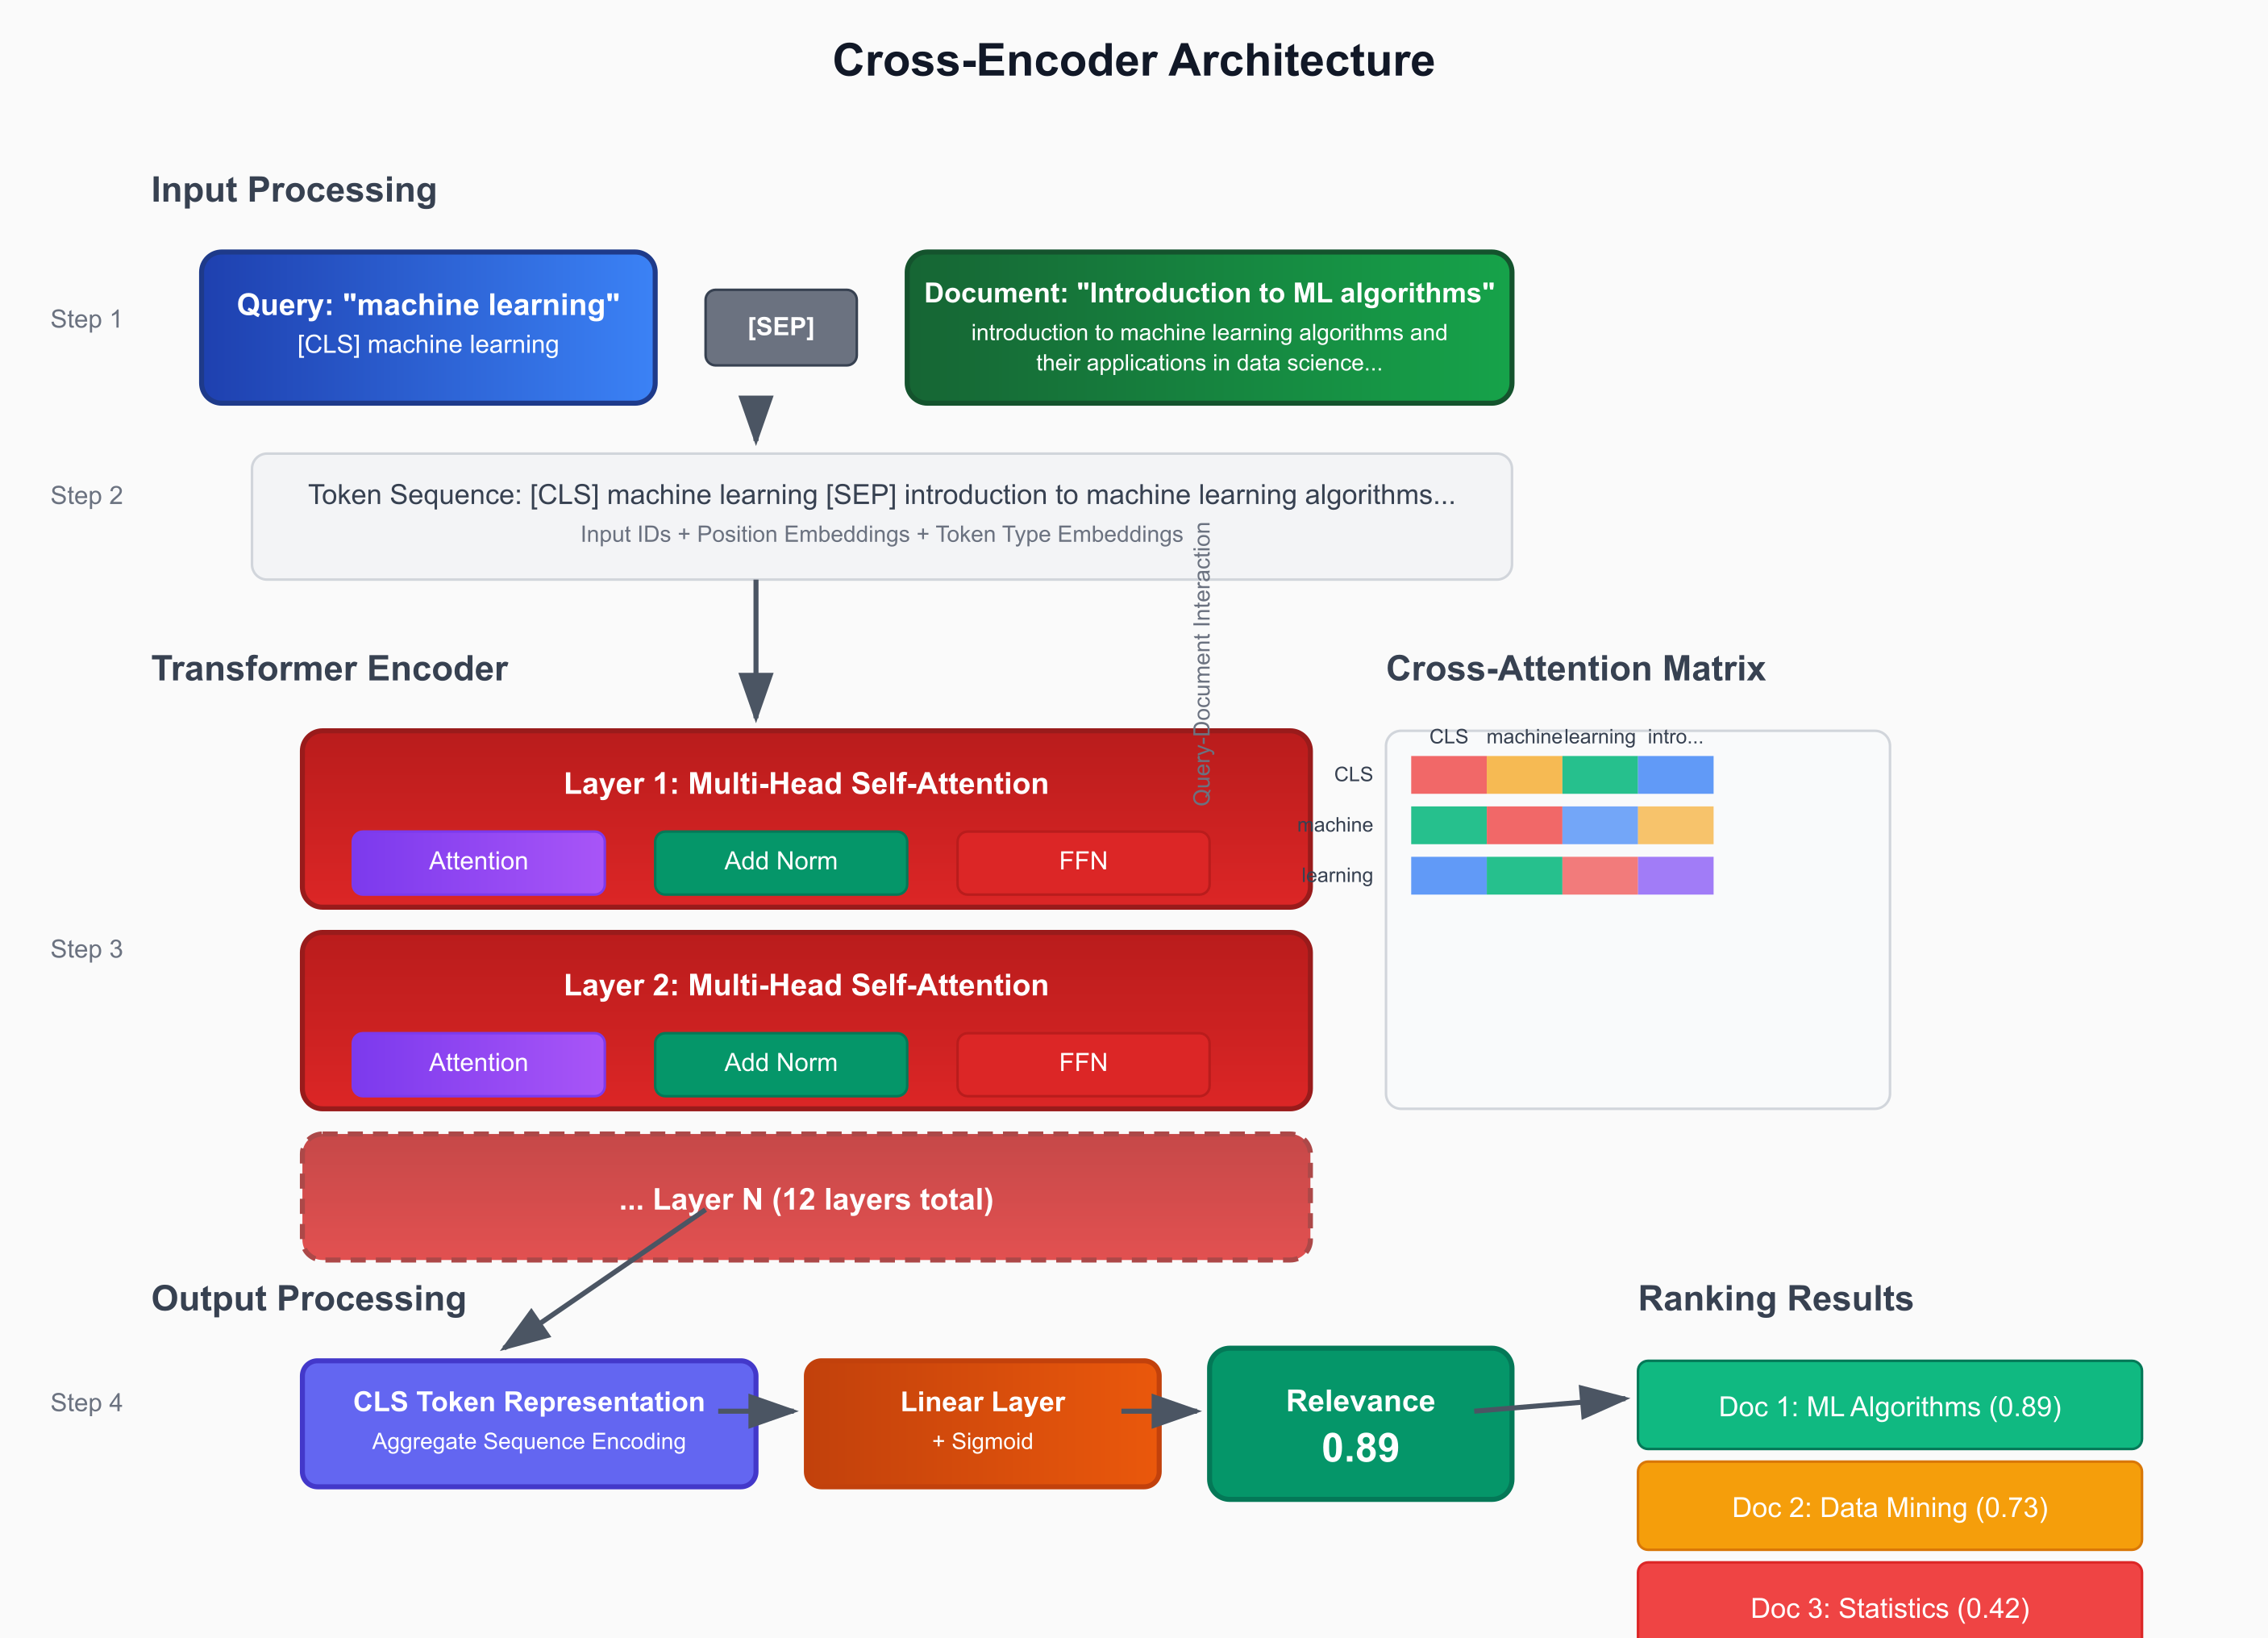
\includegraphics[width=0.8\textwidth, height=5cm, keepaspectratio]{Figures/cross_encoder_archi.png}
    \caption{Cross-Encoder Architecture for Query-Document Reranking.}
    \label{fig:Cross-Encoder-Architecture}
\end{figure}

\section{Optimization Strategies}

Cross-encoder effectiveness depends on optimization strategies during fine-tuning. While AdamW \cite{loshchilov2019decoupled} has been the standard choice, the Lion optimizer \cite{chen2023symbolic} presents a novel approach using sign-based momentum: \texttt{update = sign(momentum) * learning\_rate}. This simplification offers potential memory efficiency and different convergence characteristics compared to traditional adaptive methods.

\section{Research Objectives}

This research conducts a comprehensive comparative analysis of Lion and AdamW optimizers for cross-encoder models in information retrieval. Our primary objectives are:

\begin{enumerate}
    \item \textbf{Systematic Evaluation}: Compare Lion and AdamW across three transformer architectures (MiniLM, GTE, ModernBERT)
    \item \textbf{Comprehensive Benchmarking}: Evaluate performance using standard IR metrics on TREC DL 2019 and MS MARCO
    \item \textbf{Training Dynamics Analysis}: Investigate convergence patterns and stability across training epochs
    \item \textbf{Practical Guidelines}: Provide evidence-based recommendations for optimizer selection
\end{enumerate}

\subsection{Expected Contributions}
\begin{itemize}
\item Empirical evidence comparing Lion and AdamW optimizers across multiple architectures
\item Optimization guidelines for cross-encoder training in information retrieval
\item Analysis of training efficiency and convergence characteristics
\end{itemize}

\section{Methodology Overview}

We employ systematic experimentation across three transformer architectures representing different performance-efficiency trade-offs: MiniLM (efficient baseline), GTE (extended context), and ModernBERT (state-of-the-art). Experiments utilize standardized datasets (MS MARCO \cite{DBLP:journals/corr/NguyenRSGTMD16} for training, TREC DL 2019 \cite{craswell2020overview} for evaluation) with cloud infrastructure (Modal platform \cite{modal_labs}, NVIDIA A100-80GB GPUs) ensuring reproducible results. Comprehensive tracking through Weights \& Biases \cite{wandb2020} enables detailed training dynamics analysis.

\section{Thesis Organization}

This thesis systematically presents research methodology, experimental results, and implications:
\textbf{Chapter 2}: Literature review on cross-encoder architectures and optimization algorithms
\textbf{Chapter 3}: Research gaps and proposed comparative evaluation approach  
\textbf{Chapter 4}: Experimental methodology and implementation details
\textbf{Chapter 5}: Comprehensive results with training dynamics and statistical analysis
\textbf{Chapter 6}: Key findings, implications, and future research directions

The thesis contributes empirical insights into optimizer selection for cross-encoder architectures with implications for search engines, question-answering systems, and information retrieval applications where ranking quality is paramount.
